\subsection{Paper \I}

In \Cref{sec:screening-rules}, we demonstrated the considerable effect that screening rules have had on sparse regression problems in the large-\(p\) setting. As a result, the papers by \textcite{elghaoui2010} and \textcite{tibshirani2012} led to a surge in interest for screening rules for the lasso and its derivatives, including the elastic net. For SLOPE, however, there existed no screening rule until our work in this paper, in which we introduced the \emph{strong screening rule for SLOPE}~\parencite{larsson2020b}.

A key contribution in our paper is the development of a practical characterization of the subdifferential for the sorted \(\ell_1\) norm, from which we derive an effective algorithm for implementing the screening rule in practice. As in the cas of the strong rule for the lasso, we too demonstrate remarkable boosts in performance for fitting SLOPE~(\Cref{tab:strong-screening-slope}). The net result is a considerable extension in reach for SLOPE in the high-dimensional setting.

\begin{table}[hbtp]
  \caption{Benchmarks measuring wall-clock time for four datasets: \data{dorothea}~\parencite{guyon2004}, \data{e2006-tfidf}~\parencite{frandi2015}, \data{news20}~\parencite{lang1995}, and \data{physician}~\parencite{deb1997}, fit with different models using either the strong screening rule or no rule}
  \label{tab:strong-screening-slope}
  \centering
  \small
  \begin{tabular}[t]{%
      l
      l
      S[table-format=4.0]
      S[table-format=6.0]
      S[table-format=5.0]
      S[table-format=4.0]
    }
    \toprule
    \multicolumn{1}{c}{} & \multicolumn{1}{c}{} & \multicolumn{1}{c}{} & \multicolumn{1}{c}{} & \multicolumn{2}{c}{{Time (s)}}               \\
    \cmidrule(l{3pt}r{3pt}){5-6}
    Dataset              & Model                & $n$                  & $p$                  & {No screening}                 & {Screening} \\
    \midrule
    dorothea             & Logistic             & 800                  & 88119                & 914                            & 14          \\
    e2006-tfidf          & Least squares        & 3308                 & 150358               & 43353                          & 4944        \\
    news20               & Multinomial          & 1000                 & 62061                & 5485                           & 517         \\
    physician            & Poisson              & 4406                 & 25                   & 34                             & 34          \\
    \bottomrule
  \end{tabular}
\end{table}

\subsection{Paper \II}

As we saw in \Cref{sec:screening-rules}, screening rules are particularly effective when they are sequential, that is, operate along the regularization path. But another possibility that had previously not been explored is the idea of screening not only for the next step on the path, but for \emph{all} of the remaining steps as well. This is the idea behind \emph{look-ahead screening rules}, which we introduce in this short paper~\parencite{larsson2021}. We employ this idea for the Gap-Safe screening rule~\parencite{ndiaye2017}, which, as the name suggests, is a safe screening rule. This means that if a feature is screened out, it is guaranteed to be zero in the solution.
% TODO: add a reference to gap safe rule

In \Cref{fig:paper2-highlight}, we illustrate the effectiveness of look-ahead screening for the lasso path at the first step for the \data{leukemia} dataset. What the plot indicates is that many features can be safely exempt from model fitting for a range of steps on the path. They only need to be re-screened at the first grey square for each given feature, for instance at step 14 for the first feature.

\begin{figure}[tpb]
  \centering
  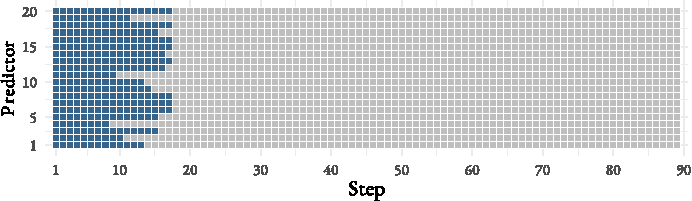
\includegraphics[]{figures/paper2-highlight.pdf}
  \caption{%
    Look-ahead screening for the lasso at the first step on the path for the \data{leukemia} dataset. The plot shows a random sample of 20 features. Blue squares indicate that the corresponding feature can be discarded for those steps on the lasso path.
  }
  \label{fig:paper2-highlight}
\end{figure}

In the paper, we show that this effect has sizeable consequences for the computation time required for fitting the full path.

\subsection{Paper \III}

Even though the strong rule for the lasso is highly effective in general, there is one area in which it struggles, namely, when features are highly correlated. \textcite{tibshirani2012} in fact noted this themselves and forwarded it as the main motivation for using the working-set strategy (where the model is initially fit using the ever-active set, rather than the strong set).

The reason for this is that the strong rule, and every other screening rules we know of, ignores information about the gradient of the correlation vector \(\vec{c}\), even though it contains useful information about the structure of the path. Looking at \Cref{fig:strong-rule}, for instance, we see that the strong rule bound is indifferent to the slopes of the correlation vectors. This is the motivation for the \emph{Hessian screening rule} that we introduce in the third paper of the thesis~\parencite{larsson2022b}. The name stems from the fact that we use second-order information about the optimization problem, which involves the Hessian matrix \(\mat{X}^\intercal\mat{X}\). The rule offers a better estimate of the correlation vector~(\Cref{fig:paper3-highlight}), which in practice leads to better screening performance.

\begin{figure}[tpb]
  \centering
  \pgfplotsset{width=11.5cm,height=9cm}
  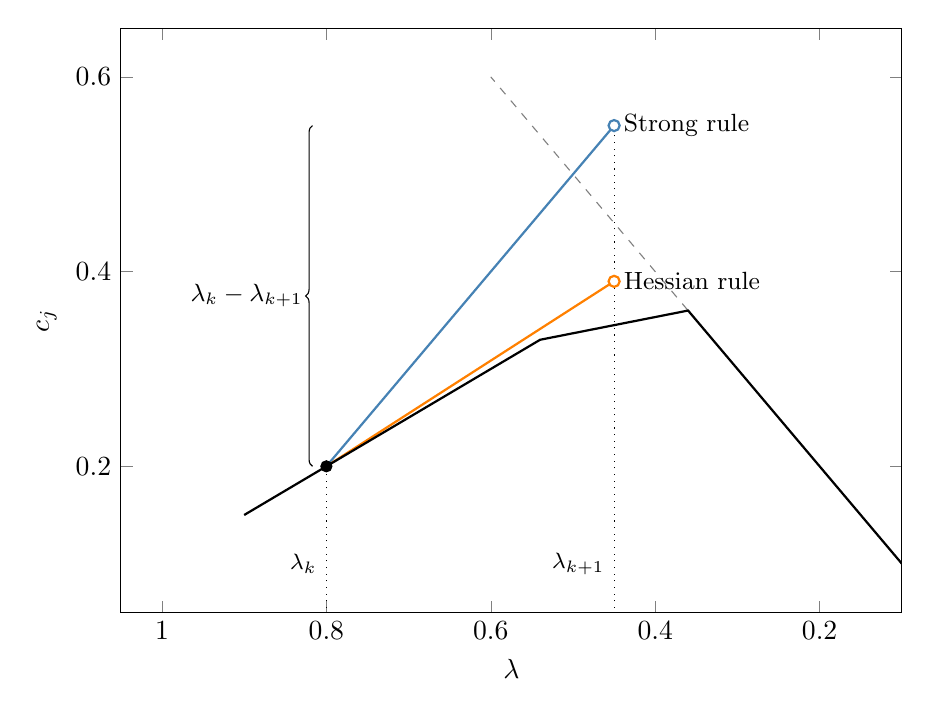
\begin{tikzpicture}
  \begin{axis}[
      ylabel = \(c_j\),
      xlabel = \(\lambda\),
      xmin = 0.1,
      xmax = 1.05,
      ymin = 0.05,
      ymax = 0.65,
      max space between ticks = 1000pt,
      try min ticks = 5,
      x dir = reverse
    ]
    \addplot[style = dashed, color=Grey]
    coordinates {
        (0.1,0.1)
        (0.6,0.6)
      };
    \addplot[thick,color=SteelBlue]
    coordinates {
        (0.8,0.2)
        (0.45,0.55)
      };
    \addplot[thick,color=orange]
    coordinates {
        (0.8,0.2)
        (0.45,0.39)
      };
    \addplot[thick]
    coordinates {
        (0.9,0.15)
        (0.54,0.33)
        (0.36,0.36)
        (0.1,0.1)
      };
    \draw [decorate,decoration={brace},xshift=-5pt]
    (0.8,0.2) -- (0.8,0.55)node [left,black,midway] {\small
      \(\lambda_{k}-\lambda_{k + 1}\)};

    \node [right] at (0.45, 0.39) {\small Hessian rule};
    \addplot[thick,mark=*,color=orange,fill=white] coordinates {(0.45,0.39)};

    \node [right] at (0.45, 0.55) {\small Strong rule};
    \addplot[thick,mark=*,color=SteelBlue,fill=white] coordinates {(0.45,0.55)};

    \addplot[mark=*] coordinates {(0.8,0.2)};

    \addplot[style=dotted]
    coordinates {
        (0.45,0.0)
        (0.45,0.55)
      };
    \addplot[style=dotted]
    coordinates {
        (0.8,0.0)
        (0.8,0.2)
      };
    \node [left] at (0.45,0.1) {\footnotesize\(\lambda_{k + 1}\)};
    \node [left] at (0.8,0.1) {\footnotesize\(\lambda_{k}\)};
  \end{axis}
\end{tikzpicture}

  \caption{%
    An illustration of the strong and Hessian screening rules for a lasso problem. We are at \(\lambda_k\) and are looking to screen features for \(\lambda_{k+1}\). The black solid line shows the path of the correlation vector for the \(j\)th feature, which is inactive (its coefficient is zero) until the point where it joins the dashed line. In blue and orange colors, we show the predicted values for \(c_j\) between \(\lambda_k\) and \(\lambda_{k+1}\). For the strong rule, the predicted value lies above the dashed line, so it is not discarded by the rule (even though it is inactive). For the Hessian rule, however, the prediction \(\hat{c}_j\) \emph{does} lie below the dashed line, and so the feature \emph{is} discarded.
  }
  \label{fig:paper3-highlight}
\end{figure}

The screening method manages to be effective, particularly when \(g\) is the least-squares objective, because of efficient updates of the Hessian matrix and its inverse. And as a bonus, the availability of these quantities also allow for adaptively tailoring the \(\lambda\) sequence in order to better approximate the true lasso path.

\subsection{Paper \IV}

The few optimization methods that we have introduced so far amount to no more than a drop in the ocean of the vast volume of research that is the field of optimization. And although we have provided a few select benchmarks of our methods, we are still far removed from any kind of comprehensive study of their comparative effectiveness. This is not just an issue of our limited overview in this thesis, but in fact a general problem for research in optimization.

The problem is that there are now so many optimization methods to examine and so many different models and datasets on which to compare them on, that it has become difficult to keep track of which methods it is that actually do best on a given problem. You can easily find a paper A that studies optimization methods X and Y on datasets I and II and conclude that X is better than Y but then find another paper B, which studies methods X, Y, and Z on datasets I and III and conclude that, actually, Y is better than X and, by the way, Z happens to be best of them all. Then, later, you find paper C, which claims that Z actually is considerably worse than X, which in fact also performs better for dataset IV. This confused state of affairs is typically the result of authors having benchmarked their methods using different hardware, programming languages for their implementations, hyperparameters for their methods, and convergence criteria, to name a few of the many possible sources of variation.

In short, there is a dire need for a framework through which this process can be made simple, reproducible, and transparent. This is the motivation behind the \pkg{benchopt} package, which we present in the fifth of this thesis' papers~\parencite{moreau2022a}.

The goal of \pkg{benchopt} is to make life easier for both researchers in optimization and users of optimization software. For a researcher who has developed a new optimization method for SLOPE, for instance, all you need to do is to write the code for your solver (optimization method) and plug it into the existing \pkg{benchopt} benchmark for SLOPE and run it. The package will then automatically compare your method with all the other methods in the benchmark and output table and plots of the results~(\Cref{fig:paper4-highlight}). If you instead are a user who is interested in using SLOPE for your applied work and want to know which algorithm to use, you can either browse the extensive database of results that other users have already uploaded or just download the benchmark and run it yourself on the data that you are interested in using it for.

\begin{figure}[htpb]
  \centering
  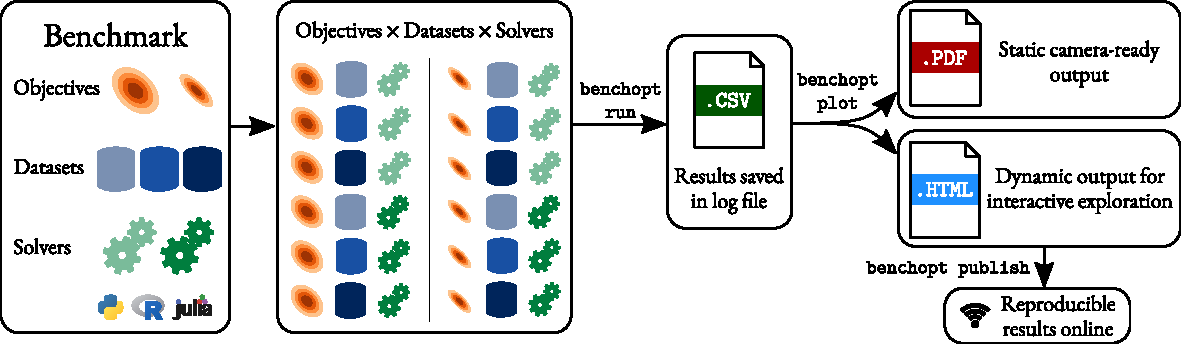
\includegraphics[width=\textwidth]{figures/benchopt_schema_objectives_with_logos.pdf}
  \caption{%
    A schematic over how a benchmark is set up and run using \pkg{benchopt}. The benchmark consists of a set of files that define objectives, datasets, and solvers. When the user runs \texttt{benchopt run}, the package combines all of the possible combinations of objectives, datasets, and solvers and outputs a neatly formatted database of the results.
    Using \texttt{benchopt plot}, the user can then easily compare the different methods through interative visualizations or produce publication-ready plots to insert directly into a paper.
    Finally, to make the results available to the \pkg{benchopt} community, the user can run \texttt{benchopt publish}, which opens up a pull-request against the public repository of benchmark results.
  }
  \label{fig:paper4-highlight}
\end{figure}

\subsection{Paper \V}

As we saw in \Cref{fig:cd-vs-pgd}, proximal coordinate descent is an efficient optimization algorithm for fitting the lasso. But as we also noted, however, it cannot handle the case when the penalty term \(h\) is non-separable, which is the case in SLOPE. In practice, this has reduced the applicability of SLOPE to large data, which is unfortunate given the many appealing properties of the model.

In paper v~\parencite{larsson2023}, however, we present a way to circumvent this issue by using a hybrid of proximal coordinate and proximal gradient descent~(\Cref{fig:paper5-highlight}). Our main discovery is that if we fix the clusters and optimize over each cluster in turn, rather than each feature, the problem becomes separable, which means that coordinate descent can be used. And if we combine this with proximal gradient descent steps, which allow us to discover the clusters, then we can guarantee convergence and at the same time benefit from the efficiency of coordinate descent.

\begin{figure}[htpb]
  \centering
  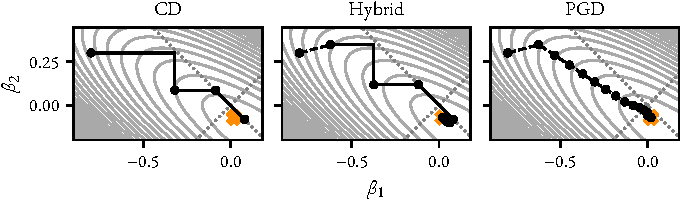
\includegraphics[]{figures/illustration_solvers_thesis.pdf}
  \caption{%
    An illustration of the hybrid coordinate descent solver we developed for SLOPE,
    showing progress until convergence for the coordinate descent solver (CD) that we use as part of the hybrid method, our hybrid method, and proximal gradient descent (PGD).
    The orange cross marks the optimum.
    Dashed lines indicate PGD steps and solid lines CD steps. Each dot marks a complete epoch, which may correspond to only a single coefficient update for the CD and hybrid solvers if the coefficients flip order. The CD algorithm converges quickly but is stuck after the third epoch. The hybrid and PGD algorithms, meanwhile, reach convergence after 67 and 156 epochs respectively.
  }
  \label{fig:paper5-highlight}
\end{figure}

\subsection{Paper \VI}

% TODO: add a reference to this paper
In the final paper of this thesis, we tackle the issue of normalization of binary features, which we touched upon in \Cref{sec:normalization}. As we saw in that section, normalization is necessary in order to put the features on the ``same scale''. What this means, however, is not clear, yet has been met mostly with neglect in the literature. We think that this is both surprising and problematic given the almost universal use of normalization in regularized methods and the apparent and large effects it has on the solution paths~(\Cref{fig:normalized-realdata-lasso-paths}).

In our paper, we begin to bridge this knowledge gap by studying normalization for the lasso and ridge regression when they are used on binary features (features that only contain values 0 or 1) or mix of binary and normally distributed features. What we find is that there is a large effect of normalization with respect to the class balance of the features: the proportion of ones to zeros (or vice versa). Both the lasso and the ridge estimators turn out to be sensitive to this class balance and, depending on the type of normalization used, have trouble recovering effects that are associated with binary features as long as their class balance is severe enough~(\Cref{fig:paper6-highlight}).

\begin{figure}[htpb]
  \centering
  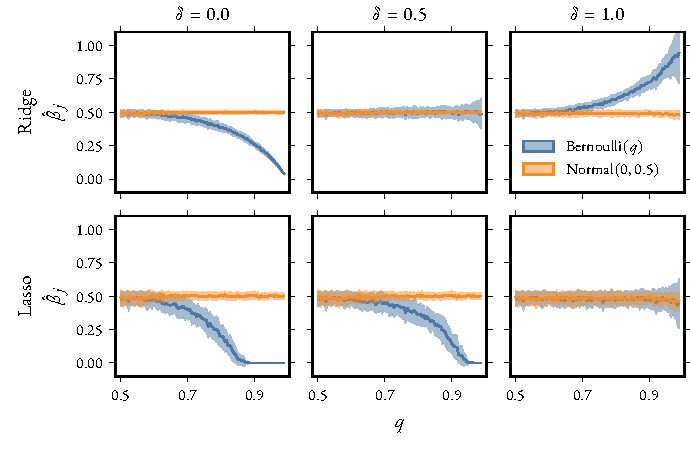
\includegraphics[]{figures/mixed_data_thesis.pdf}
  \caption{%
    Estimated coefficients from lasso and ridge regression for a two-feature problem where one of the features has a quasi-normal distribution (values deterministically set via the quantile function), with standard deviation 1/2, and the other is a binary (quasi-Bernoulli) feature with class-balance \(q\). The normal feature is standardized in every case, whereas the binary feature is scaled with \((q - q^2)^\delta\)---its variance to the power of \(\delta\). In other words, we have no scaling for \(\delta=0\), standard deviation scaling when \(\delta=1/2\), and variance-scaling when \(\delta = 1\).
  }
  \label{fig:paper6-highlight}
\end{figure}
